%capitulo1.tex
\chapter{Introducción}
\section{Historia de los medios}
%Introducción nueva
%¿Qué son las redes de sensores inalámbricos?
Tomando en cuenta que desde sus inicios la reproducción de medios siempre ha estado relacionada con los últimos avances científicos, los medios de distribución actuales tienen sus bases en los avances que datan  del siglo XIX.\\
Inicialmente los registros de audio con posibilidades de distribución aparecieron con el invento basado del fonógrafo de Thomas Alva Edison, el Gramófono de Emile Berliner, aparecido en 1887 y patentado en 1888. La diferencia con diseño original de Edison está en el medio de registro de audio con el disco de vinilo. Cabe recordar la famosa imagen de la compañía RCA Víctor del Perro escuchando la voz del amo.\\

Análogamente el registro de imágenes en movimiento apareció gracias al cinematógrafo, invento del francés Léon Bouly, y más tarde desarrollado y popularizado por los hermanos Auguste y Louis Lumière, el cual permite la grabación y reproducción del contenido con la misma máquina.\\

Esta tecnología sienta bases para la transmisión de contenidos a gran escala, broadcasting. Para el siglo XX, los avances en tecnología permiten experimentar con difusión a través del espectro de frecuencias.\\

 En los años 1920’s la radio es el medio más popular, llegando a estar presente en 40 millones de hogares estadounidenses, para dos décadas después (1950’s) ser reemplazada en popularidad por la naciente televisión.\\

	Estos medios comunicativos para la década actual (2010’s) mantienen su esencia, que es la transmisión del video y/o audio a una gran cantidad de personas. Si bien el medio por el que se transmite, la resolución, fidelidad y formato han cambiado, las bases son las mismas.\\
	
En la actualidad las transmisiones de audio y video se encuentran en un estado de transición desde medios de comunicación análogo como, por ejemplo, la radio FM, AM y la televisión PAL, NTSC, SECAM, a transmisiones digitales. El motivo de este cambio tecnológico es aprovechar de mejor manera el espectro radioeléctrico, enviando la misma o mayor información que por transmisiones análogas, pero utilizando menos recursos del espectro (Subtel Chile).\\

Otro medio de transmisión que ha tomado gran significancia en la última década es la Internet. A través de transmisiones de flujos de datos (streaming), es posible escuchar radios online, ver videos en YouTube, o utilizar servicios de películas “on-demand” como Netflix, por dar ejemplos disponibles en Chile. Todo esto siendo recibido en un computador u otro dispositivo que presente conectividad a la red.\\

Estos dispositivos alternativos tienen el peso de llevar la recepción de medios audiovisuales por un nuevo rumbo y ya están siendo considerados por las empresas que generan el contenido, al proveer salidas directas a televisores con Internet; consolas de videojuegos con navegador web o aplicaciones cliente para servicios de audio o video on-demand. Otro punto a tener en cuenta es la mayor importancia que tiene el crecimiento del consumo de dispositivos móviles como celulares o reproductores portátiles multimedia, donde se puede llegar a una audiencia aun más grande.\\

\section{Tecnología actual relacionada}

\subsection{Estado actual de las transmisiones}

Considerando que el objetivo de este trabajo tiene relación con la distribución y recepción de contenidos audiovisuales. Se presentan distintos medios funcionando actualmente.\\

Video-on-demand: es un servicio de distribución que permite a los usuarios seleccionar y ver o escuchar el contenido de video o audio de manera personalizada, ofreciendo la opción de solicitar el contenido en el momento exacto que lo desee.  La plataforma para poder reproducir el contenido se puede encontrar implementada como aplicación en un computador o a través de un dispositivo con conexión directa a al televisor y al proveedor del servicio. En Chile este servicio es provisto por la compañía VTR a través de su dispositivo D-Box, este dispositivo cumple además la función de DVR.\\

La compañía Netflix también provee este servicio, sin embargo el medio de transmisión es Internet, ofreciendo a sus clientes suscripciones que permiten el acceso al catalogo de películas.\\

En Chile se ha posicionado a partir de Septiembre de 2011, y considerando simplificar registro de nuevos usuarios, su potencial acogida nuevo usuarios se magnifica al poner a disposición de sus clientes el acceso a los contenidos a través de variadas plataformas de reproducción, como consolas de videojuegos de sobremesa, Nintendo Wii, y PlayStation 3, consolas portátiles como Nintendo 3DS, acceso vía web y aplicaciones para televisores con InternetTV. \\

Podcast: es una serie de archivos de medios digitales (audio o video) lanzados en forma periódica por episodios, este sistema permite al usuario descargar el contenido de su interés para poder verlo o escucharlo más tarde.\\

El modo de distribución se diferencia de otras formas de transferencia de internet como lo son la descarga directa al estar todos los archivos catalogados en un servidor central, este además provee a los usuarios una vía de distribución a través de RSS Feeds, que son archivos de información en XML (extended markup language) diseñados para compartir actualizaciones de sitios web, popularizados por los blogs.\\ 
El uso de RSS Feed para los podcast permite informar a las personas suscritas de nuevos contenidos, aunque no es necesario que la persona esté suscrita para obtener alguna información en especifico. 
Su uso se ha popularizado por la plataforma iTunes desarrollada por Apple, que en su versión 4.9 de 2005, abrió a una gran base de usuarios este nuevo medio de comunicación. No solo se utiliza para entregar programas de radio, sino que también documentos y programas de televisión, de manera gratuita.\\

Streaming media: este método provee constantemente datos multimedia al usuario final, que reproduce mientras tanto el servidor se encuentra entregando la información.
El nombre se refiere a que el método de entrega es continuo, sin interrupción, debido a que los datos recibidos se almacenan en un buffer de memoria que se va liberando mientas se reproduce. Es decir los datos de audio o video, no son descargados,  es un acceso directo al contenido intangible.
Un uso más reciente que se le ha dado al método streaming es lo que se llama LiveStreaming, donde el contenido a distribuir es capturado en el momento, una tranmision en vivo que es posible de ser recibida por el usuario casi al momento que ocurre gracias al flujo o stream de datos.
La base fundamental de este método de distribución, es la utilización de protocolos ligeros de la capa de transporte, como lo es UDP (User Datagram Protocol) que a diferencia del protocolo TCP (Transmission Control Protocol), no asegura la entrega en caso de fallo, permitiendo obviar los paquetes, priorizando la continuidad del flujo en el tiempo sobre la fiabilidad de los contenidos.  En la capa de aplicación se ha desarrollado un protocolo con este objetivo, toma como base la conexión mediante UDP para realizar el enlace, es llamado Real-time Transport Protocol (RTP).\\

Aun así existe un protocolo de la capa de aplicación que utiliza TCP para realizar el enlace. Este fue desarrollado originalmente por Macromedia, siendo ahora propietario Adobe Systems, el Real Time Messaging Protocol (RTMP) fue desarrollado para realizar streaming multimedia a través de TCP con baja latencia, esto lo logra gracias al envío de la mayor cantidad de información por enlace. \\
	
	De esta metodología Apple Inc. ha desarrollado un nuevo método llamado HTTP Live Streaming, que se diferencia al utilizar pedazos de audio o video  ordenados en una lista de reproducción de extensión m3u que es actualizada a medida que nuevos contenidos son creados. A diferencia del streaming nombrado anteriormente, este flujo de datos se trasmite a través del protocolo HTTP (Hypertext Transfer Protocol), el cual es de una capa superior (de aplicación) posibilitando la transferencia de los datos multimedia con un servidor web ordinario como por ejemplo Apache. Además posibilita la transmisión en redes donde firewalls o proxies bloqueen contenido ya que se enmascara como trafico de hipertexto. \\


\subsection{Almacenamiento del Contenido}

Otra tecnología que está relacionada con este tema, tiene que ver con la toma de registro de los medios recibidos. Existen en la actualidad los llamados DVR (digital video recorders), dispositivos interactivos que cumplen con la grabación de la señal de televisión o video, siendo almacenada en formato digital.\\

 Esta información queda guardada en el disco duro o memoria del sistema, para poder ser vista después. A diferencia de una antigua videograbadora, el medio de almacenamiento y el formato es digital, permitiendo tomar registro y así manipularlo mediante software.\\
 
	El concepto es aplicado en hardware para televisión e implementado en decodificadores de televisión pagada. En el caso de proveedores de cable, la transmisión es recibida por el enlace coaxial, donde el dispositivo cumple la función de decodificar la señal digital y almacenarla si posee características de DVR.\\

\subsection{Registros de Stream}

Se puede implementar este concepto de DVR en software de computadores de escritorio, desarrollando alguna aplicación que permita registrar los segmentos transmitidos por streaming para ser reproducidos en otra ocasión. \\

	Servicios de streaming bien populares como Justin.TV, UStream o Twittcam permiten transmitir video a través de sus plataformas web, y permiten la revisión del contenido tiempo después que este ha finalizado. En cierta parte este comportamiento se asemeja al DVR, pero no posibilita moverse en el tiempo mientras se transmite.\\

En Chile, se ha desarrollado una aplicación más sofisticada por parte de la empresa AltaVoz S.A. con su producto SocialStream, el cual permite retroceder y revisar el contenido mientras la transmisión se encuentra en curso. Este registro es encargado al servidor quien administra los pedazos de información multimedia, una aplicación cliente entabla conexión para realizar pedidos de la información en el tiempo que desea el usuario.
Esta característica lleva como nombre comercial TimeShift.


\section{Propuesta de Proyecto}
\subsection{El Smartphone}
Primero que todo se debe definir el concepto de Smartphone, lo cual es un teléfono portátil con conectividad a las redes celulares y que presenta características adicionales respecto a los teléfonos móviles comunes.\\

Sus bases se sientan en los siguientes conceptos:
\begin{itemize}
\item Su funcionalidad puede ser extendida a través de aplicaciones adicionales.
\item Debe poseer un teclado QWERTY físico o virtual.
\item Debe permitir estar siempre conectado a la Internet.
\end{itemize}
Considerando estos conceptos se puede encasillar como Smartphone a los teléfonos Blackberry, iPhone y Android.\\

\subsection{Trasfondo}

La mayoría de los smartphones permiten el acceso a internet a través de la red celular utilizando distintas tecnologías de transmisión de datos (no sólo WiFi), como los son actualmente EDGE y 3G. Estas se encuentran en incesante desarrollo, presentando mejoras en la velocidad de transferencia de datos.\\

La constante mejoría en la velocidad de transmisión en redes celulares ha permitido la reproducción de contenidos multimedia. Un avance similar a lo experimentado en la década de 1990 por los computadores multimedia de escritorio. En primera instancia con aplicaciones con contenido audiovisual (imagen, audio, video, texto) ejecutadas localmente, para luego llegar a recibir y transmitir este contenido a través de la world wide web.\\

Los smartphones actuales ejecutan sistemas operativos avanzados que proveen módulos de conexión  a redes, ya sea celular, WiFi, o Bluetooth, si es que el hardware lo incorpora. Además de navegadores web diseñados especialmente para estos dispositivos, con características como presentar en pantalla reducida o ajustada a la resolución, interfaz táctil, teclado numérico, etc.\\

Considerando estas 2 bases, conectividad y sistema operativo capaz, es posible implementar una aplicación que se asemeje a la experiencia en computadores de escritorio.\\


\subsection{La Problemática}
Actualmente se encuentra en desarrollo en Chile el producto SocialStream, para computadores de escritorio y aparatos de sobremesa. 
Una herramienta que permite registrar en el momento, una transmisión en vivo, ya sea de audio o video. Posibilitando al consumidor del contenido, retroceder a un punto en específico, pausar  y avanzar (limitado por el punto más reciente de la transmisión). 
A diferencia de dispositivos de sobremesa (set top boxes) como lo son TiVo u otros DVR, el registro de la transmisión es encargado al servidor que provee los contenidos a los clientes que se conectan, y esto contenidos no son guardados localmente.
Este sistema nos significan los siguientes beneficios: 
\begin{itemize}
\item Ahorro para el consumidor, espacio en sus dispositivos de almacenamiento
\item Cierto control del proveedor sobre la distribución  y copia de los contenidos
\item La posibilidad de portar a otras plataformas como consolas de videojuegos o dispositivos móviles.
\end{itemize}

Las bases de esta herramienta se fundan sobre Adobe Flash gracias a su protocolo RTMP. Y considerando el estado actual de las relaciones entre Apple y Adobe (carta de Steve Jobs, exCEO de Apple) surge nuestro principal problema:

	Las aplicaciones que cumplen la función de reproducción de los contenidos están desarrolladas en el lenguaje de programación ActionScript, propio de Adobe.

En las plataformas de escritorio y algunos smartphones, esto no significa un problema. Sin embargo los dispositivos de Apple con el sistema operativo iOS no presentan compatibilidad con estas tecnologías Flash.

\clearpage 
\begin{figure}[h!]
	\centering
	% \fbox{ } % la encierra en un cuadrado, sirve para código también
	 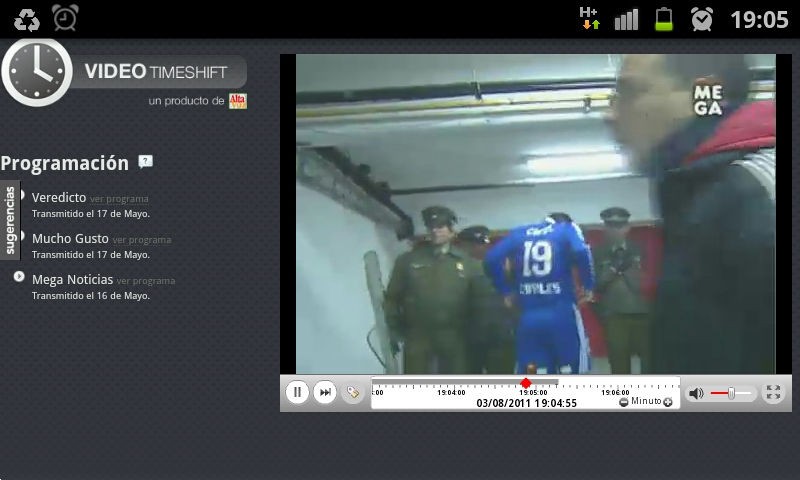
\includegraphics[scale=0.47]{imgs/sshot_Android_sstream.jpg}
 	\caption{Reproducción de SocialStream en Android OS.}
 	\label{sshot_Android_sstream}
\end{figure}
%\vspace{3cm}
\begin{figure}[h!]
	\centering
	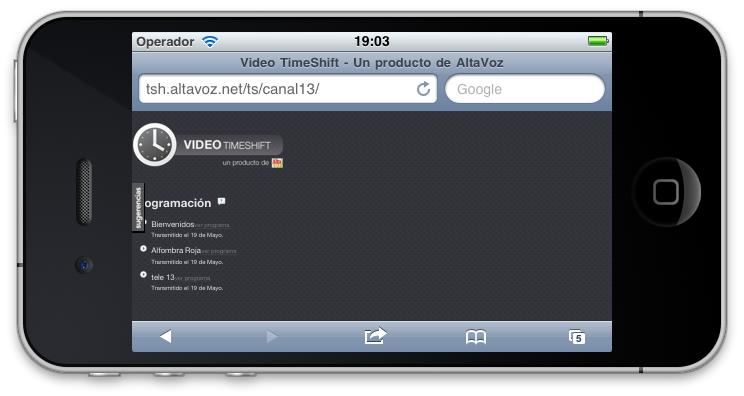
\includegraphics[scale=0.55]{imgs/sshot_iOS_sstream.png}
	\caption{Reproducción de SocialStream en iOS}
	\label{sshot_iOS_sstream}
\end{figure}

	De las figuras \ref{sshot_Android_sstream} y \ref{sshot_iOS_sstream} se puede notar claramente el problema que genera en iOS la falta de soporte de tecnologías Adobe.

\newpage
\subsection{Posibles Soluciones}

A la fecha, las herramientas de distribución de audio y/o video por streaming, están limitadas a los reproductores provistos por la interfaz de programación de aplicaciones (API) de iOS. En donde al reproducir contenido por streaming presentan la opción de retroceder la cantidad de  tiempo almacenada en el buffer de datos. \\

%\clearpage
\begin{figure}[h!]
	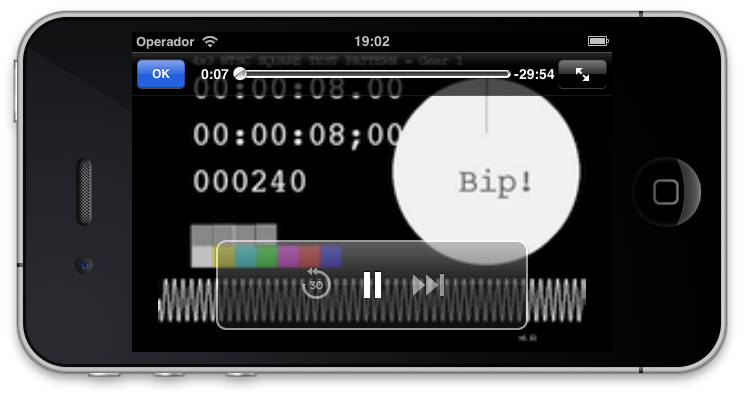
\includegraphics[scale=0.55]{imgs/sshot_iOS_hls.png}
	\caption{Reproducción de flujo video por HTTP Live Streaming}
	\label{sshot_iOS_hls}
\end{figure}

De la figura \ref{sshot_iOS_hls} se puede notar el botón a la izquierda en la barra inferior de  la pantalla, este hace retroceder en 30 segundos la reproducción.\\

Esta característica es propia del framework MediaPlayer. que simplifica de gran manera la necesidad de mostrar video en el dispositivo. Este uso también se puede aplicar para la reproducción  de  audio y video.
Se debe dejar claro que Apple es sumamente restrictivo en el uso de la API de iOS. \\
Para el desarrollo de aplicaciones, estas deben utilizar solo llamadas al sistema que estén indicadas en sus documentos guía, por lo tanto una vía para desarrollar una solución de reproductor que provea la posibilidad de saltar en la línea del tiempo de reproducción sin importar que tan larga sea la transmisión en vivo, depende de las bases MediaPlayer. \\

En la documentación actual de iOS v4.3 se encuentra AVPlayer (audio video player) [link] que pone a disposición las llamadas y manejo de datos de audio y/o video.


\subsection{Soluciones actuales}
\subsection{Pros y Contras de una nueva solución}
\subsection{El beneficio de llegar a nuevas audiencias}


% Una de las principales aplicaciones de estas redes es la construcción de sistemas de monitoreo que recolectan mediciones de variables físicas en zonas donde el monitoreo cableado representa costos muy elevados o no es posible por la falta de redes de distribución eléctrica\cite{WileyWSN}.\\
%¿Cuáles son las áreas de investigación y desarrollo de WSN?
%Las principales temas de investigación (medidas en términos de frecuencia de publicaciones) son: Despliegue, seguimiento de objetivos, localización, recolección de datos, ruteo y agregación, seguridad, protocolos de acceso al medio (MAC), acceso a bases de datos y sincronización del tiempo. Estos temas son tratados en más del cincuenta porciento del total de publicaciones\cite{WileyWSN} .\\ %buscar como continuar después de una itemezación con dos puntos y separados por comas.

%Presentar el tema del ruteo y recolección de datos
%Dentro de un sistema de recolección de datos, basado en una red de sensores inalámbricos, es necesario contar con un protocolo de ruteo que permita direccionar los datos hacia uno o varios puntos de recolección dentro de la red. Dadas las características y limitaciones de los sensores inalámbricos, el principal objetivo de estos protocolos es reducir el consumo de energía de la red, y a la vez, mantener su funcionalidad frente a las diferentes fallas que se puedan presentar\cite{WSNSurvey}.\\

%IR DE LO GENERAL A LO PARTICULAR!
%El capítulo de introducción debe comenzar explicando que son las 	WSNs.
%\section{Redes de sensores inalámbricos}

%Cosas que hay que dejar claras:
%	-Es un sistema distribuído.	OK
%	-Como nacen las WNSs.
%	-Formada por motes.	OK
%	-Qué cosas permiten las WSNs y por qué las permiten

\section{Aplicaciones}
%En el mundo
De los trabajos publicados se está en conocimiento de que las redes de sensores se están aplicando en\cite{WileyWSN}: \\

\textbf{Alerta de desastres}: La aplicación más recurrente en esta área es la detección de incendios, donde los dispositivos utilizan sensores de temperatura y algún sistema de localización para alertar en caso de incendio y/o entregar a los servicios de emergencia información relacionada con la distribución del incendio.\\

\textbf{Edificios inteligentes}: Principalmente, el uso de redes de sensores inalámbricos para entregar información a los sistemas de control de aire acondicionado y ventilación. También permiten la reducción de costos frente a los sistemas actuales que funcionan en su mayoría utilizando dispositivos cableados. También se han propuesto sistemas para monitorear los niveles de estrés mecánico en la estructura de los edificios construidos en territorios de alta actividad sísmica.\\

\textbf{Agricultura de precisión}: Las redes de sensores inalámbricas aplicadas a la agricultura están, generalmente, construidas para realizar mediciones de suelo: humedad, temperatura y sales. Se ha determinado que un sensor por hectárea es suficiente para obtener datos necesarios para monitorear el estado de los cultivos.\\

%En chile

%Red para monitoreo forestal
En Chile, durante los años 2006 y 2007 se desarrolló el proyecto ''Redes inalámbricas de sensores para la detección de incendios forestales y monitoreo de variables de estado de combustibles para el recurso forestal de la Región de Valparaíso''\cite{ProyectoForestal}. El proyecto fue desarrollado en conjunto por ADDERE Ltda., CONAF, Universidad de Concepción, Forestal ACE Internacional S.A., ONEMI, CORMA y la Agencia Chilena del Espacio. El objetivo de este proyecto era monitorear el estado de los combustibles forestales y detectar los posibles focos de incendio en tiempo real, debido a que anualmente se queman más de seis mil hectáreas sólo en la Región de Valparaíso, causando pérdidas materiales por más de cincuenta millones de dólares.\\

%Wiseconn
Wiseconn es una empresa chilena que se ha dedicado a desarrollar productos para la agricultura de precisión utilizando redes de sensores inalámbricos. Actualmente utilizan tecnología basada en la especificación Zigbee para recolectar datos relacionados con mediciones de suelo \cite{Wiseconn}.

%Austec

\section{Protocolo de ruteo para un sistema de recolección de datos}
%\section{Visión general de los requerimientos}
%Hablar de la aplicación objetivo y cuáles son sus requerimientos 
%La implementación de un protocolo de ruteo se realiza como parte de un sistema de recolección de datos orientado a. Por ejemplo, el sistema se puede desplegar en un terreno de cultivo, donde se desee principalmente medir la temperatura y la humedad del suelo, luego concentrar esos datos en un Gateway que enviaría esos datos a través de una red ethernet a un sistema computacional que almacena, analiza y presenta esos datos a través de una aplicación web. \\

%Títulos alternativos
El objetivo de este trabajo es implementar un protocolo de ruteo multihop como parte de un sistema de recolección de datos que está construido sobre una red de sensores inalámbricos. Este sistema está orientado principalmente al monitoreo de variables físicas principalmente relacionadas con la agricultura, como la humedad y la temperatura de los suelos, en zonas de difícil acceso y que no cuentan con redes de distribución eléctrica.

\begin{figure}[H]
% \includegraphics[scale=0.625]{imgs/ArquitecturaGeneral.eps} 
\caption{Arquitectura general del sistema de recolección.}
\end{figure}

En la figura 1.1, se describe la arquitectura del sistema de recolección de datos. Este sistema tiene como objetivo principal: mover los datos desde los puntos en la red donde se realizan las mediciones, hasta el punto en la red donde los datos son concentrados y enviados por otro medio de transmisión en el camino a su destino final. Para realizar esta tarea se debe implementar una capa de red, que se encargue de controlar la topología de la red y establecer rutas para los mensajes que transportan los datos. El sistema está ideado para utilizar una red de entre 30 y 50 nodos, donde todos los nodos (excluyendo el Gateway) son energéticamente autónomos y su tiempo de operación debe alcanzar el orden de meses.

Los requerimientos establecidos para la implementación del protocolo son los siguientes:

\begin{enumerate}
\item \textbf{Rutear los mensajes hacia el Gateway:} Se debe implementar un protocolo que realice el ''mejor esfuerzo'' en transportar los mensajes desde un nodo origen, reenviar los mensajes por nodos intermedios y entregarlos al Gateway.Se debe contemplar que el nodo puede recibir mensajes de múltiples nodos en un periodo de tiempo reducido, por lo que debe de alguna manera almacenar los mensajes recibidos y enviarlos en orden, minimizando la pérdida de mensajes.\\

\item \textbf{Tolerar falla de desaparición de nodos:} En el contexto de la comunicación multi-hop son muchas las fallas e inconsistencias que se pueden generar, sin embargo, el protocolo multi-hop debe al menos tolerar la desaparición de nodos de la red, es decir, si un nodo es sacado de la red o agota su batería, entonces la red no debe dejar de funcionar y los nodos que se queden sin ruta, deben buscar otra si es que existe.\\

\item\textbf{Reducir el consumo energético:} Dado que la principal variable de diseño, en todos los aspectos, de una red de sensores inalámbricos es el consumo energético, el protocolo implementado debe realizar operaciones que permitan gestionar el consumo y alcanzar un tiempo de operación del orden de meses. \\
\end{enumerate}

En el marco de este trabajo, los objetivos generales son los siguientes:
\begin{enumerate}
  \item Informar sobre los protocolos de ruteo de mensajes para redes de sensores inalámbricos.
  \item Desarrollar una red de sensores inalámbricos, utilizando la plataforma de hardware TmoteSky.
  \item Desarrollar una aplicación para la recolección de datos de la red.
  \item Evaluar el consumo energético de la red implementada.
\end{enumerate}

 El primer objetivo se desarrolla en profundidad en el capítulo 2. El segundo objetivo se desarrolla en los capítulos 3, 4 y 5, donde se plantea un diseño de protocolo y posteriormente como se implementa éste. El tercer objetivo se desarrolla en los capítulos 3 y 5 como parte de las verificaciones del sistema. Finalmente, en el capítulo 5 se evalúa el consumo energético el protocolo.\\
 
\section{Estado del Arte}
El estado del arte para un sistema de recolección de datos se describe utilizando la siguiente estructura: primero, se revisan los algoritmos más recurrentes en la literatura orientados a la recolección de datos; segundo, se describen los algoritmos implementados para las plataformas más populares; finalmente, se describe el software y hardware de desarrollo disponible.

\subsection{Protocolo de ruteo}
Según el modelo OSI para el diseño de comunicación entre computadores, la capa de red es responsable de todo lo relacionado con entrega de paquetes de un computador origen a uno destino. Esto incluye el direccionamiento lógico de mensajes y el ruteo de paquetes a través de una o varias redes. Un componente de la implementación de la capa de red son los algoritmos de ruteo. \\

%\begin{figure}[H]
 %\centering
 %\includegraphics[scale=0.8]{imgs/PilaModeloOSI.eps}
 %\caption{Pila de red establecida por el Modelo OSI}
%\end{figure}

Los algoritmos de ruteo, son métodos que permiten definir rutas dentro de una red para transmitir paquetes de datos. La estrategia de ruteo elegida puede tener un impacto significativo en el desempeño de la red\cite{WSNSurvey}.\\

%Las redes de sensores inalámbricos son extremadamente versátiles, por lo que la forma en que éstas son desplegadas, dependerá de la naturaleza de la aplicación. Las redes pueden estar compuestas de nodos estáticos o móviles. Por ejemplo: para aplicaciones de monitoreo, los sensores son desplegados en un área y, usualmente, se mantienen estáticos mientras recolectan información; para aplicaciones en el área de la salud, los nodos pueden ser adheridos a insumos o personas para monitorear sus signos vitales, en este caso, la red debe permitir la movilidad de los nodos.\\

Un primer enfoque para diseminar datos en la red, es enviar los datos recolectados por un nodo en un salto (comunicación directa) hacia el gateway, sin embargo, si el nodo está muy lejos del gateway, puede que éste nunca reciba el mensaje. Por lo tanto, el siguiente enfoque son los protocolos multi-hop, donde varios nodos intermedios se encargan de llevar un paquete de datos desde fuente a destino. En un algoritmo multi-hop, cada nodo ejecuta el algoritmo de ruteo que determinará cuál es el próximo destino de un paquete en la red.

% \subsection{Algoritmos de ruteo propuestos en la literatura}

%En esta sección debería dar una breve reseña  de cada protocolo, con sus referencias.
%\subsection{Protocolos implementados}

%\subsection{Hardware de desarrollo}
%De lo general a lo particular
% Qué tipo de hardware existe?

%Debo incluir info sobre los motes que soportan tinyos
\subsubsection{Plataformas TinyOS}
Algunas de las plataformas de desarrollo soportadas actualmente por TinyOS 2.1 son:

\begin{center}
\begin{table}[H]
\caption{Algunas plataformas de hardware soportadas por TinyOS} 
\begin{tabular}{|l|p{10cm}|}
\hline \textbf{Plataforma} & \textbf{Descripción} \\ 

\hline Intelmote2 \cite{IntelMote2Web} &  Plataforma basada en el procesador PXA271 XScale, tranceptor CC2420, posee dos conectores de 31 y 21 pines para sensores,  e interfaz USB. Utiliza dos baterías AA\\ 

%\hline Iris \cite{IrisDatasheet} & Plataforma basada en el SoC XM2110CA de Atmel, conector de expansión de 51 pines para sensores. Utiliza dos baterías AA \\ 

\hline Mica2 \cite{Mica2Datasheet} &  Plataforma basada en el Soc de bajo consumo Atmel ATmega 128L, conector de expansión de 51 pines para sensores. Utiliza dos baterías AA. \\ 

\hline Micaz \cite{MicazDatasheet} &  Plataforma basada en el Soc de bajo consumo Atmel ATmega 128L, conector de expansión de 51 pines para sensores. \\ 

%\hline Shimmer \cite{ShimmerWiki} &  Plataforma diseñada para vestir, basada en el microprocesador de bajo consumo MSP430F1611. Incorpora un tranceptor Bluetooth WML-C46A y un tranceptor CC2420. Posee un lector de tarjetas Micro-SD para almacenamiento masivo. Incluye un acelerómetro de 3-ejes. Tiene una batería recargable de Ion-Litio integrada.\\ 

\hline TelosB (TmoteSky) \cite{TelosBDatasheet} & Plataforma basada en el microcontrolador de bajo consumo MSP430, utiliza el transceptor CC2420, incluye sensores de radiación solar total y radiación fotosintétizable. Utiliza dos pilas AA.  \\ 

%\hline Tinynode \cite{TinyNodeWeb} &  Plataforma basada en el microcontrolador de bajo consumo MSP430, utiliza el tranceptor de bajo consumo Xemics  XE 1205, conector de expansión de 31 pines para conectar sensores e interfaces de comunicación serial.\\ 
\hline 

\end{tabular}

\end{table} 
\end{center}
%Se omiten Mica, Mica2dot, eyesIFX  y telos a porque parece que están descontinuados


\subsubsection{Plataformas Zigbee}
Texas Instruments es uno de los principales impulsores de esta tecnología, ellos comercializan las siguientes plataformas de desarrollo.
%Debo incluir info sobre los motes que soportan Zigbee, simpliciti.
\begin{table}[H]
\centering
\caption{Plataformas de desarrollo Zigbee}
\begin{tabular}{|l|p{10cm}|}
\hline \textbf{Plataforma} & \textbf{Descripción} \\ 
\hline CC2430ZDK & Kit de desarrollo para redes Zigbee que incluye tarjetas de desarrollo para el SoC CC2430. Poseen interfaz USB y utiliza dos baterías AA. \\ 
\hline CC2530ZDK & Kit de desarrollo para redes Zigbee que incluye tarjetas de desarrollo para el SoC CC2530. Poseen interfaz USB y utiliza dos baterías AA.\\ 
\hline 
\end{tabular} 
\end{table}

\subsubsection{Otras plataformas}
A continuación se describen otras plataformas para redes de sensores inalámbricos.
\begin{table}[H]
\centering
\caption{Otras plataformas de desarrollo para redes de sensores inalámbricos}
\begin{tabular}{|l|p{10cm}|}
\hline \textbf{Plataforma} & \textbf{Descripción} \\ 
%\hline ATAVRRZ201 \cite{ATAVRRZ201}& Kit de desarrollo para redes Zigbee basado en el microcontrolador ATMega1281V y el tranceptor AT86RF230.\\ 
\hline AVR Raven & Kit de demostración para redes Zigbee que incluye un dispositivo que integra tres chips: el ATmega3290P para manejar los dispositivos I/O; el ATMega1284P para ejecutar la pila de comunicación; y la radio AT86RF230. Estas tarjetas incluyen un Display, un parlante, micrófono, memoria flash, reloj de tiempo real, botones y switchs. Utiliza una batería de tipo botón o alimentación externa desde 5V hasta 12V.\\
\hline EM430F6137RF900 & Plataforma basada en el SoC CC430, que integra un MSP430 y una radio CC1100 en un chip. Incluye un conector para Display LCD que se distribuye junto con la plataforma. Puede utilizar dos baterías AAA. \\ 
\hline ez430 Chronos & Plataforma de desarrollo embebida en un reloj deportivo. Esta plataforma está basada en el SoC CC2430, e incluye acelerómetro y sensor de presión, además de los de temperatura y voltaje del CC430. Utiliza una batería de celda tipo botón.\\ 
\hline SunSpot & Los dispositivos SunSPOTs son motes para redes de sensores inalámbricos desarrollados por Sun Microsystems. Estos dispositvos utilizan el estándar IEEE 802.15.4 para comunicación inalámbrica y tienen integrada la máquina virtual de Java (Squawk). Además, cada SunSPOT cuenta con acelerómetro, sensor de temperatura, sensor de luz, 8 leds tri-color y 2 switches. \\ 
\hline 
\end{tabular} 
\end{table}


\subsection{Software para redes de sensores inalámbricos}
%TinyOS, ZStack, SimpliciTI, etc
%Breve descripción de tinyOS e indicación para revisar el anexo XX.
\subsubsection{TinyOS}
TinyOS es un sistema operativo embebido de código abierto, diseñado especialmente para desarrollar aplicaciones para redes de sensores inalámbricos. Su desarrollo comenzó en la Universidad de Berkeley a fines de los años 90 y actualmente su desarrollo está a cargo de la TinyOS Alliance. TinyOS está diseñado para permitir concurrencia, operación con recursos limitados, soporte de un rango amplio de aplicaciones y hardware, y adaptación a la evolución del hardware. TinyOS es un sistema conducido por eventos  programado en NesC, un dialecto derivado de C que reduce el consumo de memoria, utiliza la programación orientada a componentes y provee la detección de ``race conditions''. \\

\subsubsection{Contiki}
Contiki es otro sistema operativo embebido de código abierto, diseñado para ser portable, multi-tarea, y con un consumo de memoria reducido. Contiki es desarrollado en el Swedish Instute of Computer Science y actualmente cuenta con desarrolladores de la industria como Cisco y Atmel. Este sistema provee comunicación vía IPv4 e IPv6, mediante la utilización de una versión reducida de la pila IP diseñada para microcontroladores. Además, provee un sistema de archivos para almacenar información en la memoria flash de los nodos. Actualmente, Contiki soporta el hardware TmoteSky (Telosb).

%Breve descripción de ZStack, basarse en pagina de ti del zstack
\subsubsection{Z-Stack}
Z-Stack es la implementación del standard Zigbee desarrollada por Texas Instruments para su portafolio de hardware compatible con el IEEE 802.15.4. La versión actual implementa las especificaciones Zigbee 2007, Zigbee Pro y Zigbee 2006. Los chips que soportan este software son: CC2530, MSP430+CC2520, CC2430 y MSP430+CC2420. 	Esta implementación se construye sobre el sistema operativo OSAL que provee herramientas como Tasks (Tareas), Timers y un manejo más amigable de las interrupciones. Es importante destacar que ninguna de las versiones implementa la topología Cluster-Tree para una red completa de sensores independientes energéticamente que propone la especificación.

%Breve descripción de SimpliciTI, basarse en pagina de ti de simpliciti
\subsubsection{SimpliciTI}
SimpliciTI es un protocolo de bajo consumo desarrollado por Texas Instruments 	para sus productos Sub-1GHz y portafolio compatible con el IEEE 802.15.4. Es un protocolo reducido que permite implementar redes con topología estrella, donde dispositivos always-on  coordinan la red. A diferencia de Z-Stack, SimpliciTI no está construido sobre un sistema operativo, por lo que no provee abstracciones de hardware ni herramientas de programación como OSAL.	

%Breve descripción de la de los sunspots, basarse en documentacion
\subsubsection{Java y SunSpot}
Los SunSPOTs son distribuidos junto a un kit de desarrollo que trae las herramientas, tutoriales y ejemplos necesarios para realizar la programación de estos dispositivos. El kit incluye el IDE Netbeans y todos los accesorios (compiladores, depuradores, interfaz de software para comunicación USB) incorporados al IDE. Estos dispositivos son programados en JAVA, utilizando la máquina virtual Squawk para ejecutar el bytecode en el dispositivo. La máquina virtual java Squawk es un desarrollo experimental de código abierto con el objetivo de acelerar la portabilidad y funcionalidad de la máquina virtual Java. Las principales características que permiten su implementación para un dispositivo embebido, son el tamaño reducido del bytecode generado (35\%  a 45\% de una clase equivalente en J2ME)  y una arquitectura que permite ahorrar memoria del dispositivo.

%Breve descripción de alguna otra de otro fabricante..freescale o atmel.



